\documentclass[aspectratio=169,xcolor=dvipsnames]{beamer}

\usetheme{Madrid}
\usecolortheme{seahorse}

% Packages
\usepackage[utf8]{inputenc}
\usepackage[T1]{fontenc}
\usepackage[french]{babel}
\usepackage{graphicx}
\usepackage{amsmath}
\usepackage{amsfonts}
\usepackage{amssymb}
\usepackage{booktabs}
\usepackage{listings}
\usepackage{xcolor}
\usepackage{tikz}
\usepackage{adjustbox}

% Configuration listings
\lstset{
    basicstyle=\ttfamily\scriptsize,
    breaklines=true,
    frame=single,
    backgroundcolor=\color{gray!10},
    keywordstyle=\color{blue}\bfseries,
    commentstyle=\color{green!60!black},
    stringstyle=\color{red},
    showstringspaces=false,
    columns=flexible
}

\lstdefinelanguage{pseudo}{
    morekeywords={Pour,chaque,epoch,mini-batch,Forward,Loss,Backward,Update,Model,LossFn},
    sensitive=false,
    morecomment=[l]{//}
}

% Informations
\title[MLP et Autodiff sur MNIST]{Implémentation from scratch d'un MLP\\et moteur d'autodifférenciation\\appliqués à MNIST}
\author{Jianye Shi, Hao Qian, Xiang Bian, Abdennour Boulmis}
\institute{M1 CHPS -- Université Paris-Saclay\\UVSQ 2025/2026}
\date{\today}

% Logo
\logo{
\includegraphics[height=0.8cm]{Images/Logo_UVSQ.jpg}}

\begin{document}

% Page de titre
\begin{frame}
\titlepage
\end{frame}

% Sommaire
\begin{frame}{Plan de la présentation}
\tableofcontents

\vspace{0.5cm}

\begin{block}{Déroulement}
\begin{itemize}
    \item Contexte et problématique (5 min)
    \item Architecture et implémentation (8 min)
    \item Résultats expérimentaux (10 min)
    \item Conclusion et perspectives (2 min)
\end{itemize}
\end{block}
\end{frame}

% ============================================================
\section{Introduction et Contexte}
% ============================================================

\begin{frame}{Contexte du projet}
\begin{block}{Objectifs}
\begin{itemize}
    \item Implémenter \textbf{from scratch} un réseau de neurones (MLP) en C++
    \item Développer un moteur de différenciation automatique
    \item Appliquer au dataset MNIST (reconnaissance de chiffres manuscrits)
    \item Double focus : \textbf{Machine Learning} + \textbf{High Performance Computing}
\end{itemize}
\end{block}

\vspace{0.3cm}

\begin{columns}[T]
\column{0.5\textwidth}
\textbf{Aspect ML}
\begin{itemize}
    \item Rétropropagation
    \item Optimisation (SGD)
    \item Convergence
\end{itemize}

\column{0.5\textwidth}
\textbf{Aspect HPC}
\begin{itemize}
    \item Optimisation bas niveau
    \item Parallélisme (OpenMP)
    \item BLAS, vectorisation
\end{itemize}
\end{columns}
\end{frame}

\begin{frame}{Le problème MNIST}
\begin{columns}[c]
\column{0.6\textwidth}
\begin{itemize}
    \item \textbf{Dataset classique} de classification
    \item Images $28 \times 28$ pixels (784 features)
    \item 10 classes (chiffres 0-9)
    \item 60,000 images d'entraînement
    \item 10,000 images de test
\end{itemize}

\vspace{0.5cm}
\textbf{Notre approche :} MLP simple mais complet
\begin{itemize}
    \item Architecture : 784 → 128 → 10
    \item Activation ReLU
    \item Loss CrossEntropy
\end{itemize}

\column{0.4\textwidth}
\centering
\textit{[Image MNIST]}\\
\vspace{0.3cm}
Objectif : $\sim$98\% de précision
\end{columns}
\end{frame}

% ============================================================
\section{Fondements théoriques}
% ============================================================

\begin{frame}{Architecture du MLP}
\begin{columns}[c]
\column{0.48\textwidth}
\begin{figure}
\centering

\includegraphics[width=\linewidth,height=0.6\textheight,keepaspectratio]{Images/LayersOfMLP.png}
\caption{Structure hiérarchique du MLP}
\end{figure}

\column{0.48\textwidth}
\textbf{Propagation avant (Forward)}
\vspace{0.2cm}

Entrée : $X \in \mathbb{R}^{N \times 784}$

Couche cachée : 
\[H = \sigma(XW_1 + b_1)\]

Sortie : 
\[Y = \text{softmax}(HW_2 + b_2)\]

\vspace{0.3cm}
\textbf{Calcul par mini-batch}
\begin{itemize}
    \item Vectorisation des opérations
    \item Exploitation du parallélisme
    \item $N$ exemples simultanément
\end{itemize}
\end{columns}
\end{frame}

\begin{frame}{Autodifférenciation et Graphe de Calcul}
\begin{columns}[c]
\column{0.55\textwidth}
\textbf{Principe du DAG (Directed Acyclic Graph)}
\begin{itemize}
    \item Chaque opération = un nœud
    \item Stockage des valeurs intermédiaires
    \item Calcul automatique des gradients
\end{itemize}

\vspace{0.3cm}
\textbf{Règle de la chaîne}
\[
\frac{\partial L}{\partial x} = \frac{\partial L}{\partial y} \cdot \frac{\partial y}{\partial x}
\]

\vspace{0.3cm}
\textbf{Backward pass}
\begin{itemize}
    \item Tri topologique du graphe
    \item Propagation des gradients
    \item Mise à jour des paramètres
\end{itemize}

\column{0.45\textwidth}
\begin{exampleblock}{Exemple simple}
\begin{align*}
z &= x \cdot w \\
y &= z + b \\
L &= y^2
\end{align*}

\vspace{0.2cm}
Gradients :
\begin{align*}
\frac{\partial L}{\partial y} &= 2y \\
\frac{\partial L}{\partial z} &= \frac{\partial L}{\partial y} \\
\frac{\partial L}{\partial w} &= \frac{\partial L}{\partial z} \cdot x
\end{align*}
\end{exampleblock}
\end{columns}
\end{frame}

% ============================================================
\section{Implémentation}
% ============================================================

\begin{frame}{Architecture logicielle}
\begin{center}
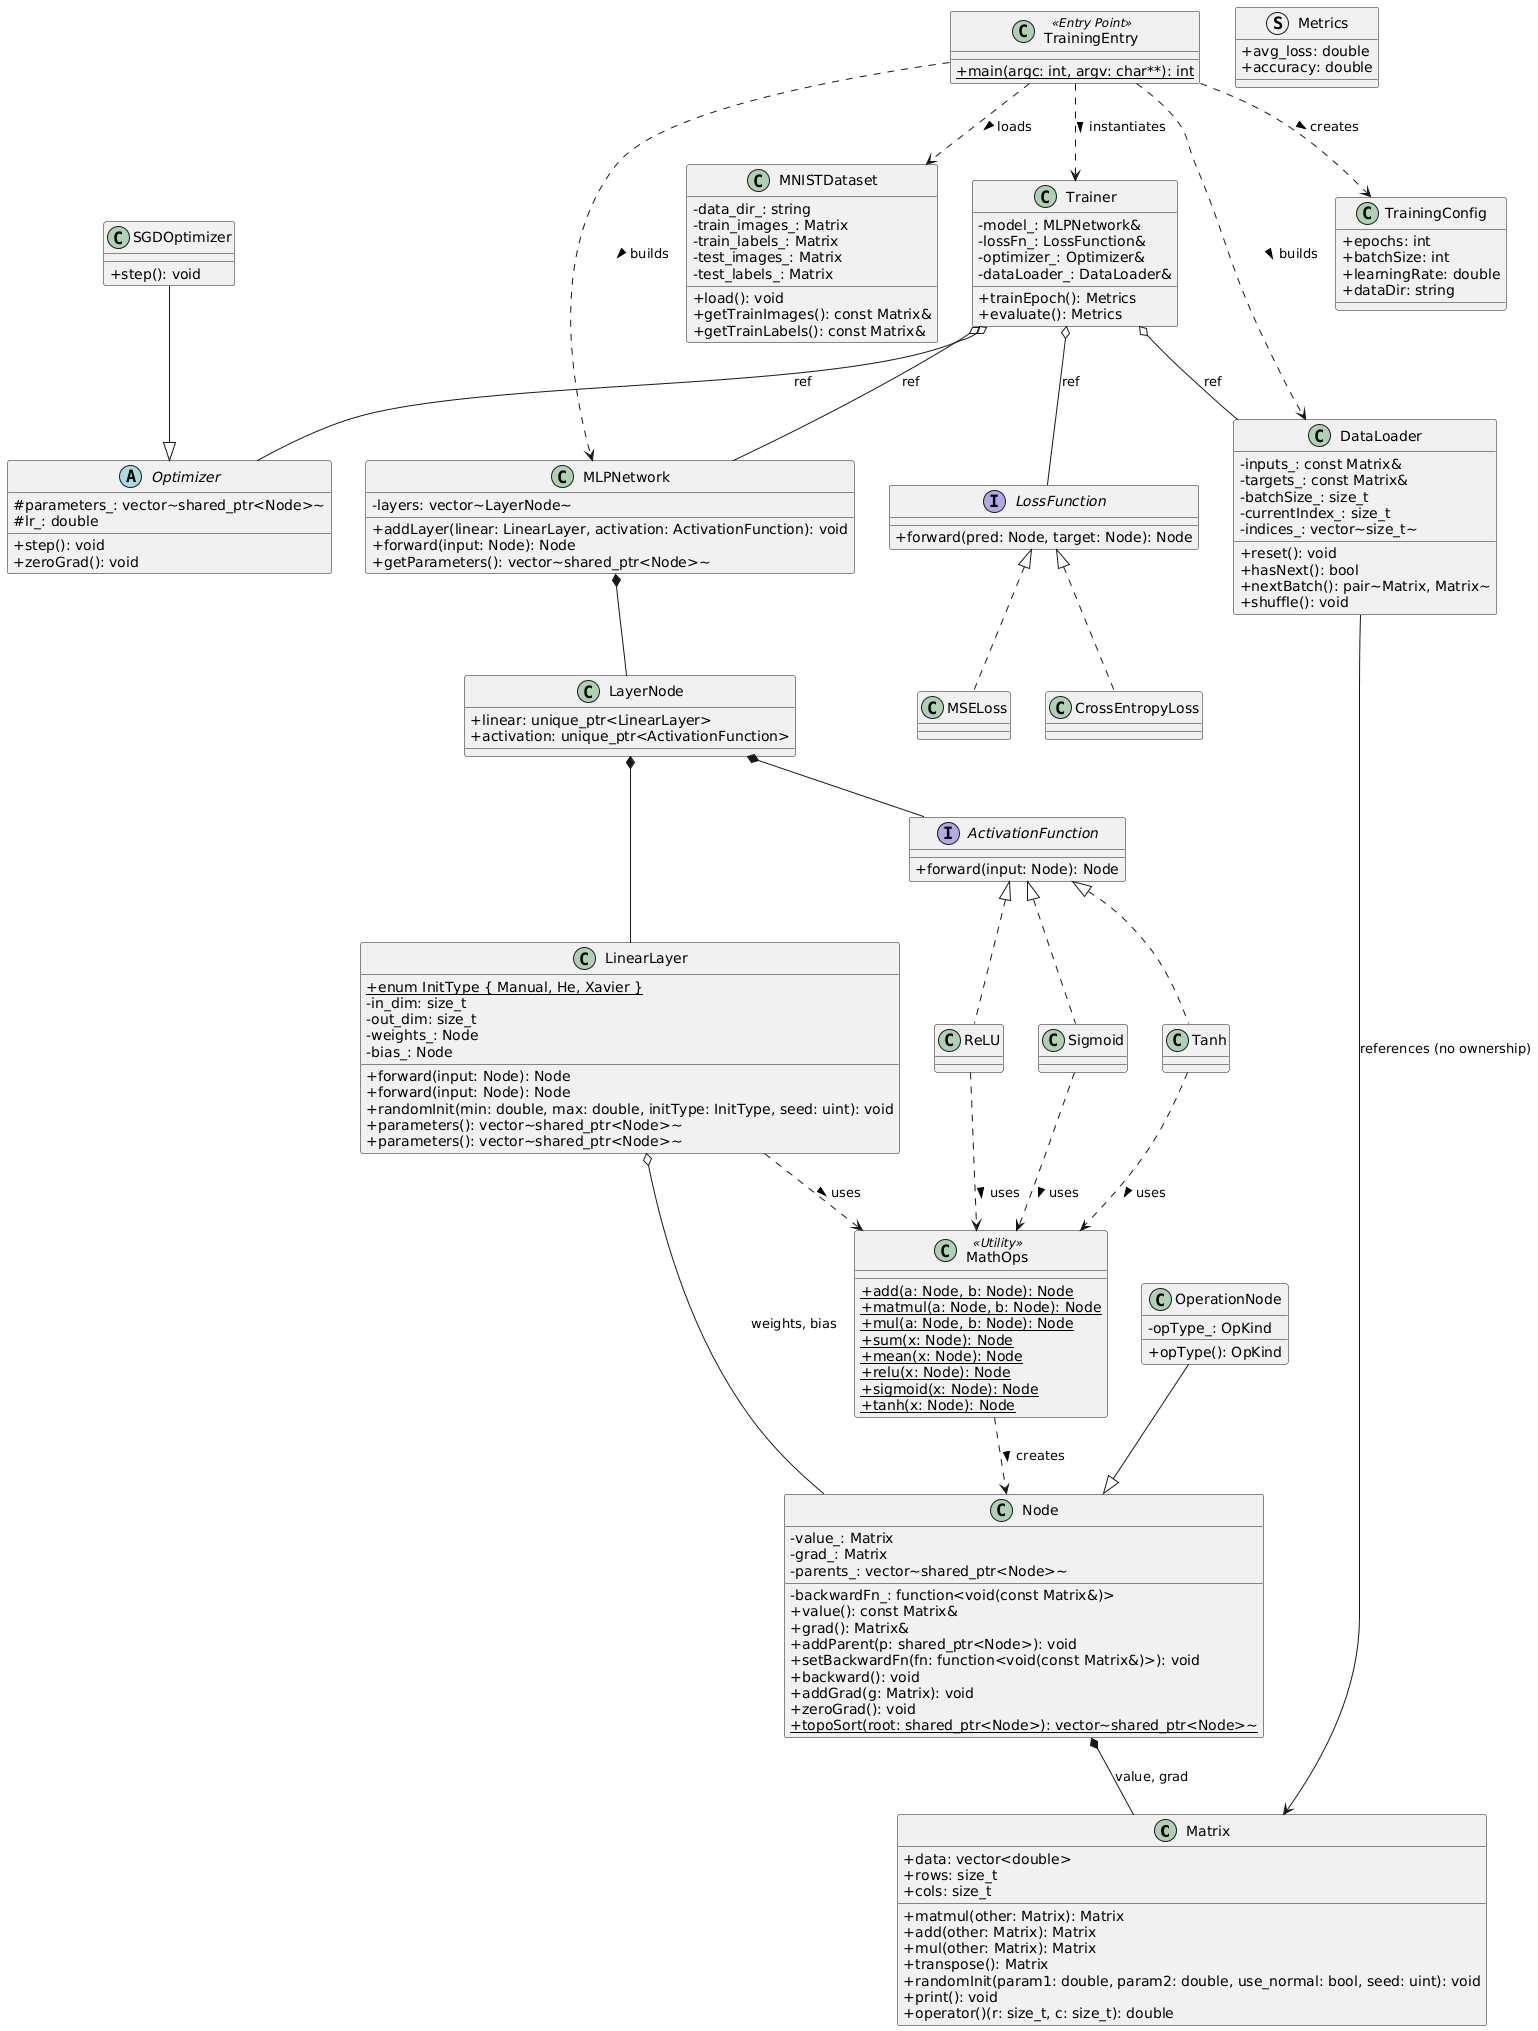
\includegraphics[width=0.9\textwidth,height=0.65\textheight,keepaspectratio]{Images/conception_detaillee.png}
\end{center}
\vspace{-0.15cm}
\begin{center}
\small
Architecture en couches : du calcul matriciel au pipeline d'entraînement
\end{center}
\end{frame}

\begin{frame}[fragile]{Construction du modèle MLPNetwork}
{\small
Le réseau est construit par composition modulaire avec support multi-couches :
}

\vspace{0.1cm}

\begin{lstlisting}[language=C++]
// Architecture flexible (network.cpp)
MLPNetwork MLPNetwork::createMultiHidden(
    int input_dim, const std::vector<int>& hidden_dims,
    int output_dim, const std::string& activation_name,
    const std::string& init_name, unsigned int seed
) {
    MLPNetwork net;
    int prev = input_dim;
    
    // Couches cachees : prev -> h + activation
    for (int h : hidden_dims) {
        net.addLayer(
            makeLinear(prev, h, init_name, seed),
            makeActivation(activation_name)
        );
        prev = h;
    }
    
    // Couche de sortie : logits, sans activation
    net.addLayer(makeLinear(prev, output_dim, init_name, seed),
                 nullptr);
    return net;
}
\end{lstlisting}

\vspace{0.1cm}

{\small
\textbf{Exemple} : \texttt{--hidden\_sizes 256,128,64} crée 784→256→128→64→10
}
\end{frame}

\begin{frame}{Noyau de calcul : Matrix}
\begin{block}{Choix de conception}
\begin{itemize}
    \item Stockage contigu : \texttt{std::vector<double>}
    \item Optimisation de la localité cache
    \item Support de la vectorisation (SIMD)
\end{itemize}
\end{block}

\vspace{0.2cm}

\begin{columns}[T]
\column{0.48\textwidth}
{\small
\textbf{Implémentations \texttt{matmul}}
\begin{itemize}
    \item Naïve ($ijk$) : pédagogique
    \item Réordonnée ($ikj$) : cache-friendly
    \item Bloquée : optimisation cache
    \item OpenMP : parallélisation
    \item BLAS : référence optimisée
\end{itemize}

\vspace{0.1cm}
\textbf{Sélection runtime}\\
Variable : \texttt{MATMUL\_IMPL}
}

\column{0.48\textwidth}
{\small
\textbf{Initialisation des poids}
\begin{itemize}
    \item \textbf{He} : pour ReLU\\
    $\text{Var}(W) = 2/n_{in}$
    \item \textbf{Xavier} : pour Sigmoid/Tanh\\
    $\text{Var}(W) = 1/n_{in}$
    \item \textbf{Manual} : $[-0.1, 0.1]$
\end{itemize}

\vspace{0.1cm}
\textbf{Reproductibilité}\\
Graine contrôlée (\texttt{--seed})
}
\end{columns}
\end{frame}

\begin{frame}[fragile]{Moteur d'autodiff : Node et MathOps}
\begin{block}{Implémentation via Lambdas C++}
\begin{itemize}
    \item \texttt{std::shared\_ptr<Node>} : gestion mémoire automatique
    \item Capture du contexte par closures
    \item Pas de classes dédiées par opération
\end{itemize}
\end{block}

\vspace{0.1cm}

\begin{lstlisting}[language=C++]
// Exemple : Multiplication y = a * b (math_ops.cpp)
Node::Ptr mul(const Node::Ptr& a, const Node::Ptr& b) {
    Matrix out = a->value().mul(b->value());
    auto node = std::make_shared<OperationNode>(
        OpKind::MUL, out, {a, b}
    );
    
    node->setBackwardFn([a, b](const Matrix& grad) {
        a->addGrad(grad.mul(b->value())); // dL/da = grad * b
        b->addGrad(grad.mul(a->value())); // dL/db = grad * a
    });
    return node;
}
\end{lstlisting}

\vspace{0.1cm}

{\small
\begin{columns}[T]
\column{0.5\textwidth}
\textbf{Avantages}
\begin{itemize}
    \item Tri topologique (DFS)
    \item Broadcasting automatique
\end{itemize}

\column{0.5\textwidth}
\textbf{Performance}
\begin{itemize}
    \item Sans récursion profonde
    \item Typage via \texttt{OpKind}
\end{itemize}
\end{columns}
}
\end{frame}

\begin{frame}[fragile]{Pipeline d'entraînement}
\begin{columns}[T]
\column{0.48\textwidth}
{\small
\textbf{Modules principaux}
\begin{itemize}
    \item \texttt{LinearLayer} : $y = xW + b$
    \item \texttt{ActivationFunction}\\
    ReLU, Sigmoid, Tanh
    \item \texttt{LossFunction}\\
    MSE, CrossEntropy
    \item \texttt{Optimizer} : SGD
    \item \texttt{DataLoader} : mini-batch
\end{itemize}
}

\column{0.48\textwidth}
{\small
\textbf{Boucle d'entraînement}
\begin{enumerate}
    \item Charger mini-batch $(X, Y)$
    \item \textbf{Forward} : $\hat{Y} = \text{Model}(X)$
    \item \textbf{Loss} : $L = \text{Loss}(\hat{Y}, Y)$
    \item \textbf{Backward} : calcul gradients
    \item \textbf{Update} : $W \leftarrow W - \eta \nabla W$
\end{enumerate}
}
\end{columns}

\vspace{0.2cm}

\begin{lstlisting}[language=C++]
// Implementation SGD (optimizer.cpp)
void SGDOptimizer::step() {
    for (auto& p : parameters_) {
        Matrix& val = const_cast<Matrix&>(p->value());
        const Matrix& grad = p->grad();
        for(size_t i=0; i<val.data.size(); ++i) {
            val.data[i] -= lr_ * grad.data[i]; // W = W - eta * grad
        }
    }
}
\end{lstlisting}

\vspace{0.1cm}

\begin{alertblock}{\small CrossEntropy optimisée}
{\scriptsize Softmax stable + gradient : $\nabla_z L = p - y$}
\end{alertblock}
\end{frame}

% ============================================================
\section{Expérimentations}
% ============================================================

\begin{frame}{Configuration expérimentale}
\begin{columns}[T]
\column{0.5\textwidth}
\textbf{Matériel}
\begin{itemize}
    \item AMD Ryzen 9 8940HX
    \item 16 cœurs / 32 threads
    \item 30 GiB RAM
    \item Cache L3 : 64 MiB
\end{itemize}

\vspace{0.3cm}
\textbf{Logiciel}
\begin{itemize}
    \item Fedora Linux 42
    \item GCC 15.2.1
    \item Flags : \texttt{-O3 -march=native}
\end{itemize}

\column{0.5\textwidth}
\textbf{Protocole rigoureux}
\begin{itemize}
    \item \textbf{Fréquence verrouillée} : 4.0 GHz
    \item \textbf{Affinité CPU} : \texttt{taskset}
    \item \textbf{Warm-up} : 5 itérations
    \item \textbf{Graine fixée} : reproductibilité
\end{itemize}

\vspace{0.3cm}
\begin{alertblock}{Objectif}
Mesures fiables et reproductibles pour comparer les optimisations
\end{alertblock}
\end{columns}
\end{frame}

\begin{frame}{Passage à l'échelle (Thread Scaling)}
\vspace{-0.2cm}
\begin{columns}[c]
\column{0.49\textwidth}
\begin{center}
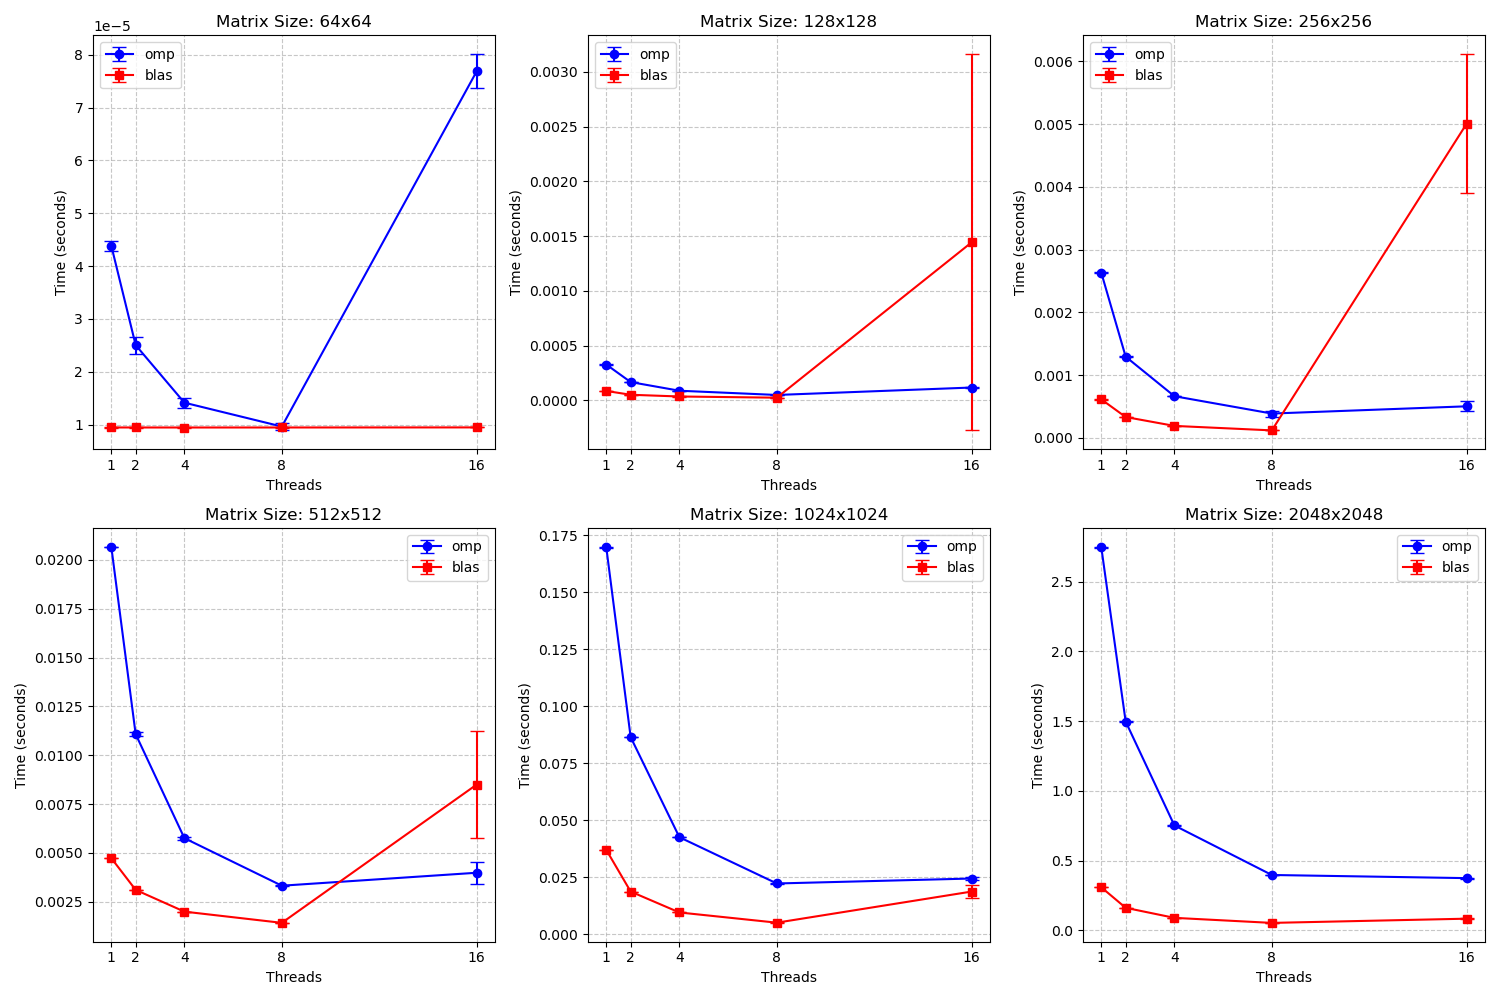
\includegraphics[width=\linewidth,height=0.46\textheight,keepaspectratio]{Images/scaling_plot.png}
\vspace{-0.15cm}
{\scriptsize Temps d'exécution vs threads}
\end{center}

\column{0.49\textwidth}
\begin{center}
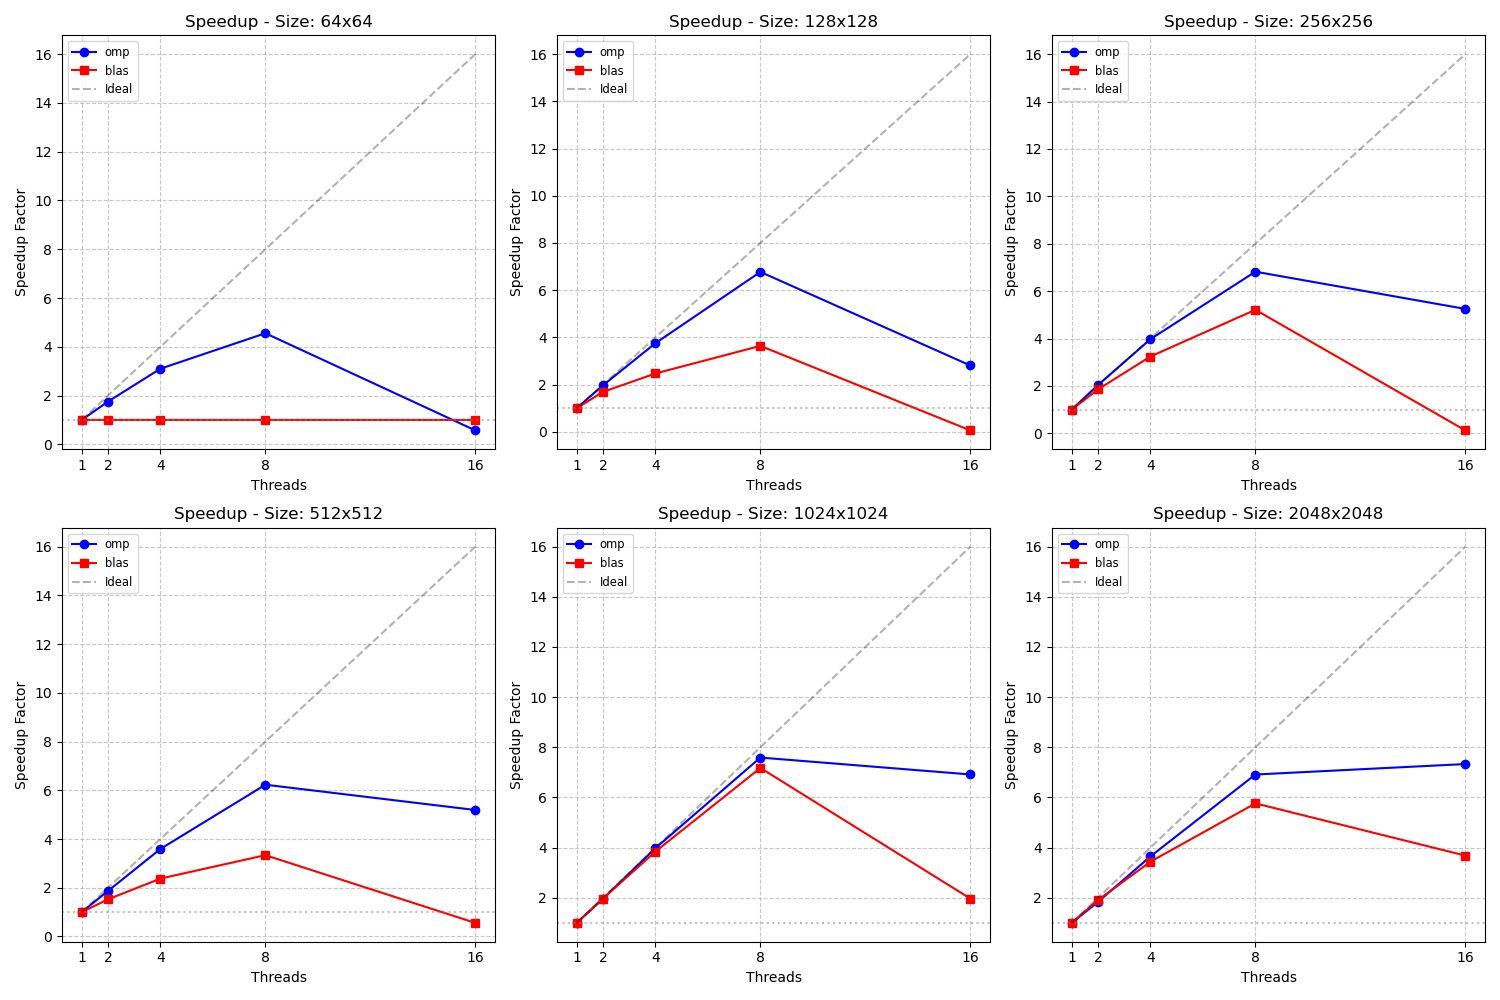
\includegraphics[width=\linewidth,height=0.46\textheight,keepaspectratio]{Images/scaling_speedup_plot.png}
\vspace{-0.15cm}
{\scriptsize Speedup vs threads}
\end{center}
\end{columns}

\vspace{0.25cm}
{\small
\begin{itemize}
    \item \textbf{64×64} : surcoût > gain au-delà de 8 threads
    \item \textbf{2048×2048} : limité par bande passante mémoire
    \item \textbf{Optimum} : 8 threads = cœurs physiques
\end{itemize}
}
\end{frame}

\begin{frame}{Hiérarchie des performances}
\vspace{-0.3cm}
\begin{center}
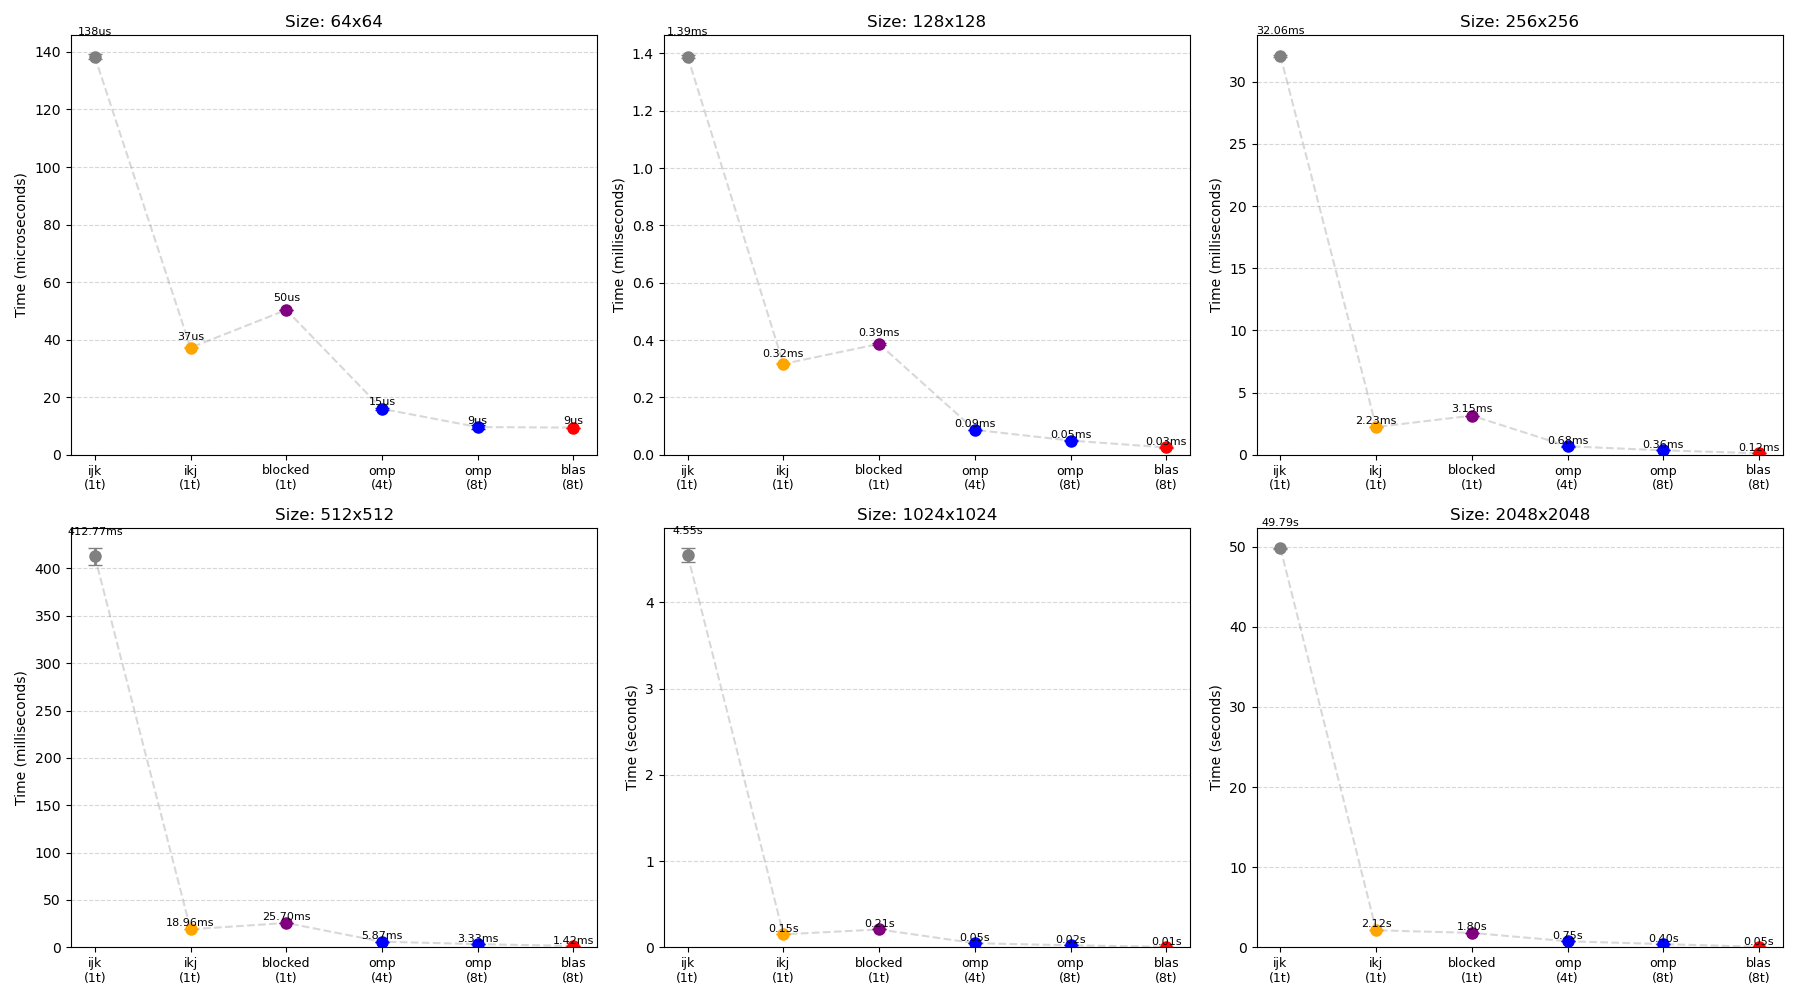
\includegraphics[width=0.82\textwidth,height=0.5\textheight,keepaspectratio]{Images/comparison_grid_plot.png}
\vspace{-0.15cm}
{\scriptsize Comparaison des implémentations matmul (matrices 2048×2048)}
\end{center}

\vspace{0.2cm}

\begin{center}
{\small
\begin{tabular}{lccc}
\toprule
\textbf{Version} & \textbf{Temps (ms)} & \textbf{Speedup} & \textbf{Technique} \\
\midrule
Naïf ($ijk$) & $\sim$3000 & 1× & Baseline \\
Réordonné ($ikj$) & $\sim$800 & 3.75× & Localité cache \\
OpenMP (8T) & $\sim$150 & 20× & Parallélisation \\
\textbf{BLAS} & $\sim$\textbf{15} & \textbf{200×} & \textbf{Vect. + SIMD} \\
\bottomrule
\end{tabular}
}
\end{center}
\end{frame}

\begin{frame}{Profiling et Loi d'Amdahl}
\vspace{-0.2cm}
\begin{columns}[c]
\column{0.54\textwidth}
{\small
\textbf{Avant optimisation (Naïf)}
\begin{itemize}
    \item \texttt{matmul} : \textcolor{red}{\textbf{96\%}}
    \item Compute-bound
    \item Temps/époque : 13.27s
\end{itemize}

\vspace{0.3cm}
\textbf{Après optimisation (BLAS)}
\begin{itemize}
    \item \texttt{matmul} : \textcolor{green}{\textbf{<1\%}}
    \item I/O données : 43\%
    \item Allocations : 29\%
    \item Temps/époque : 1.74s
\end{itemize}
}

\column{0.44\textwidth}
\begin{center}
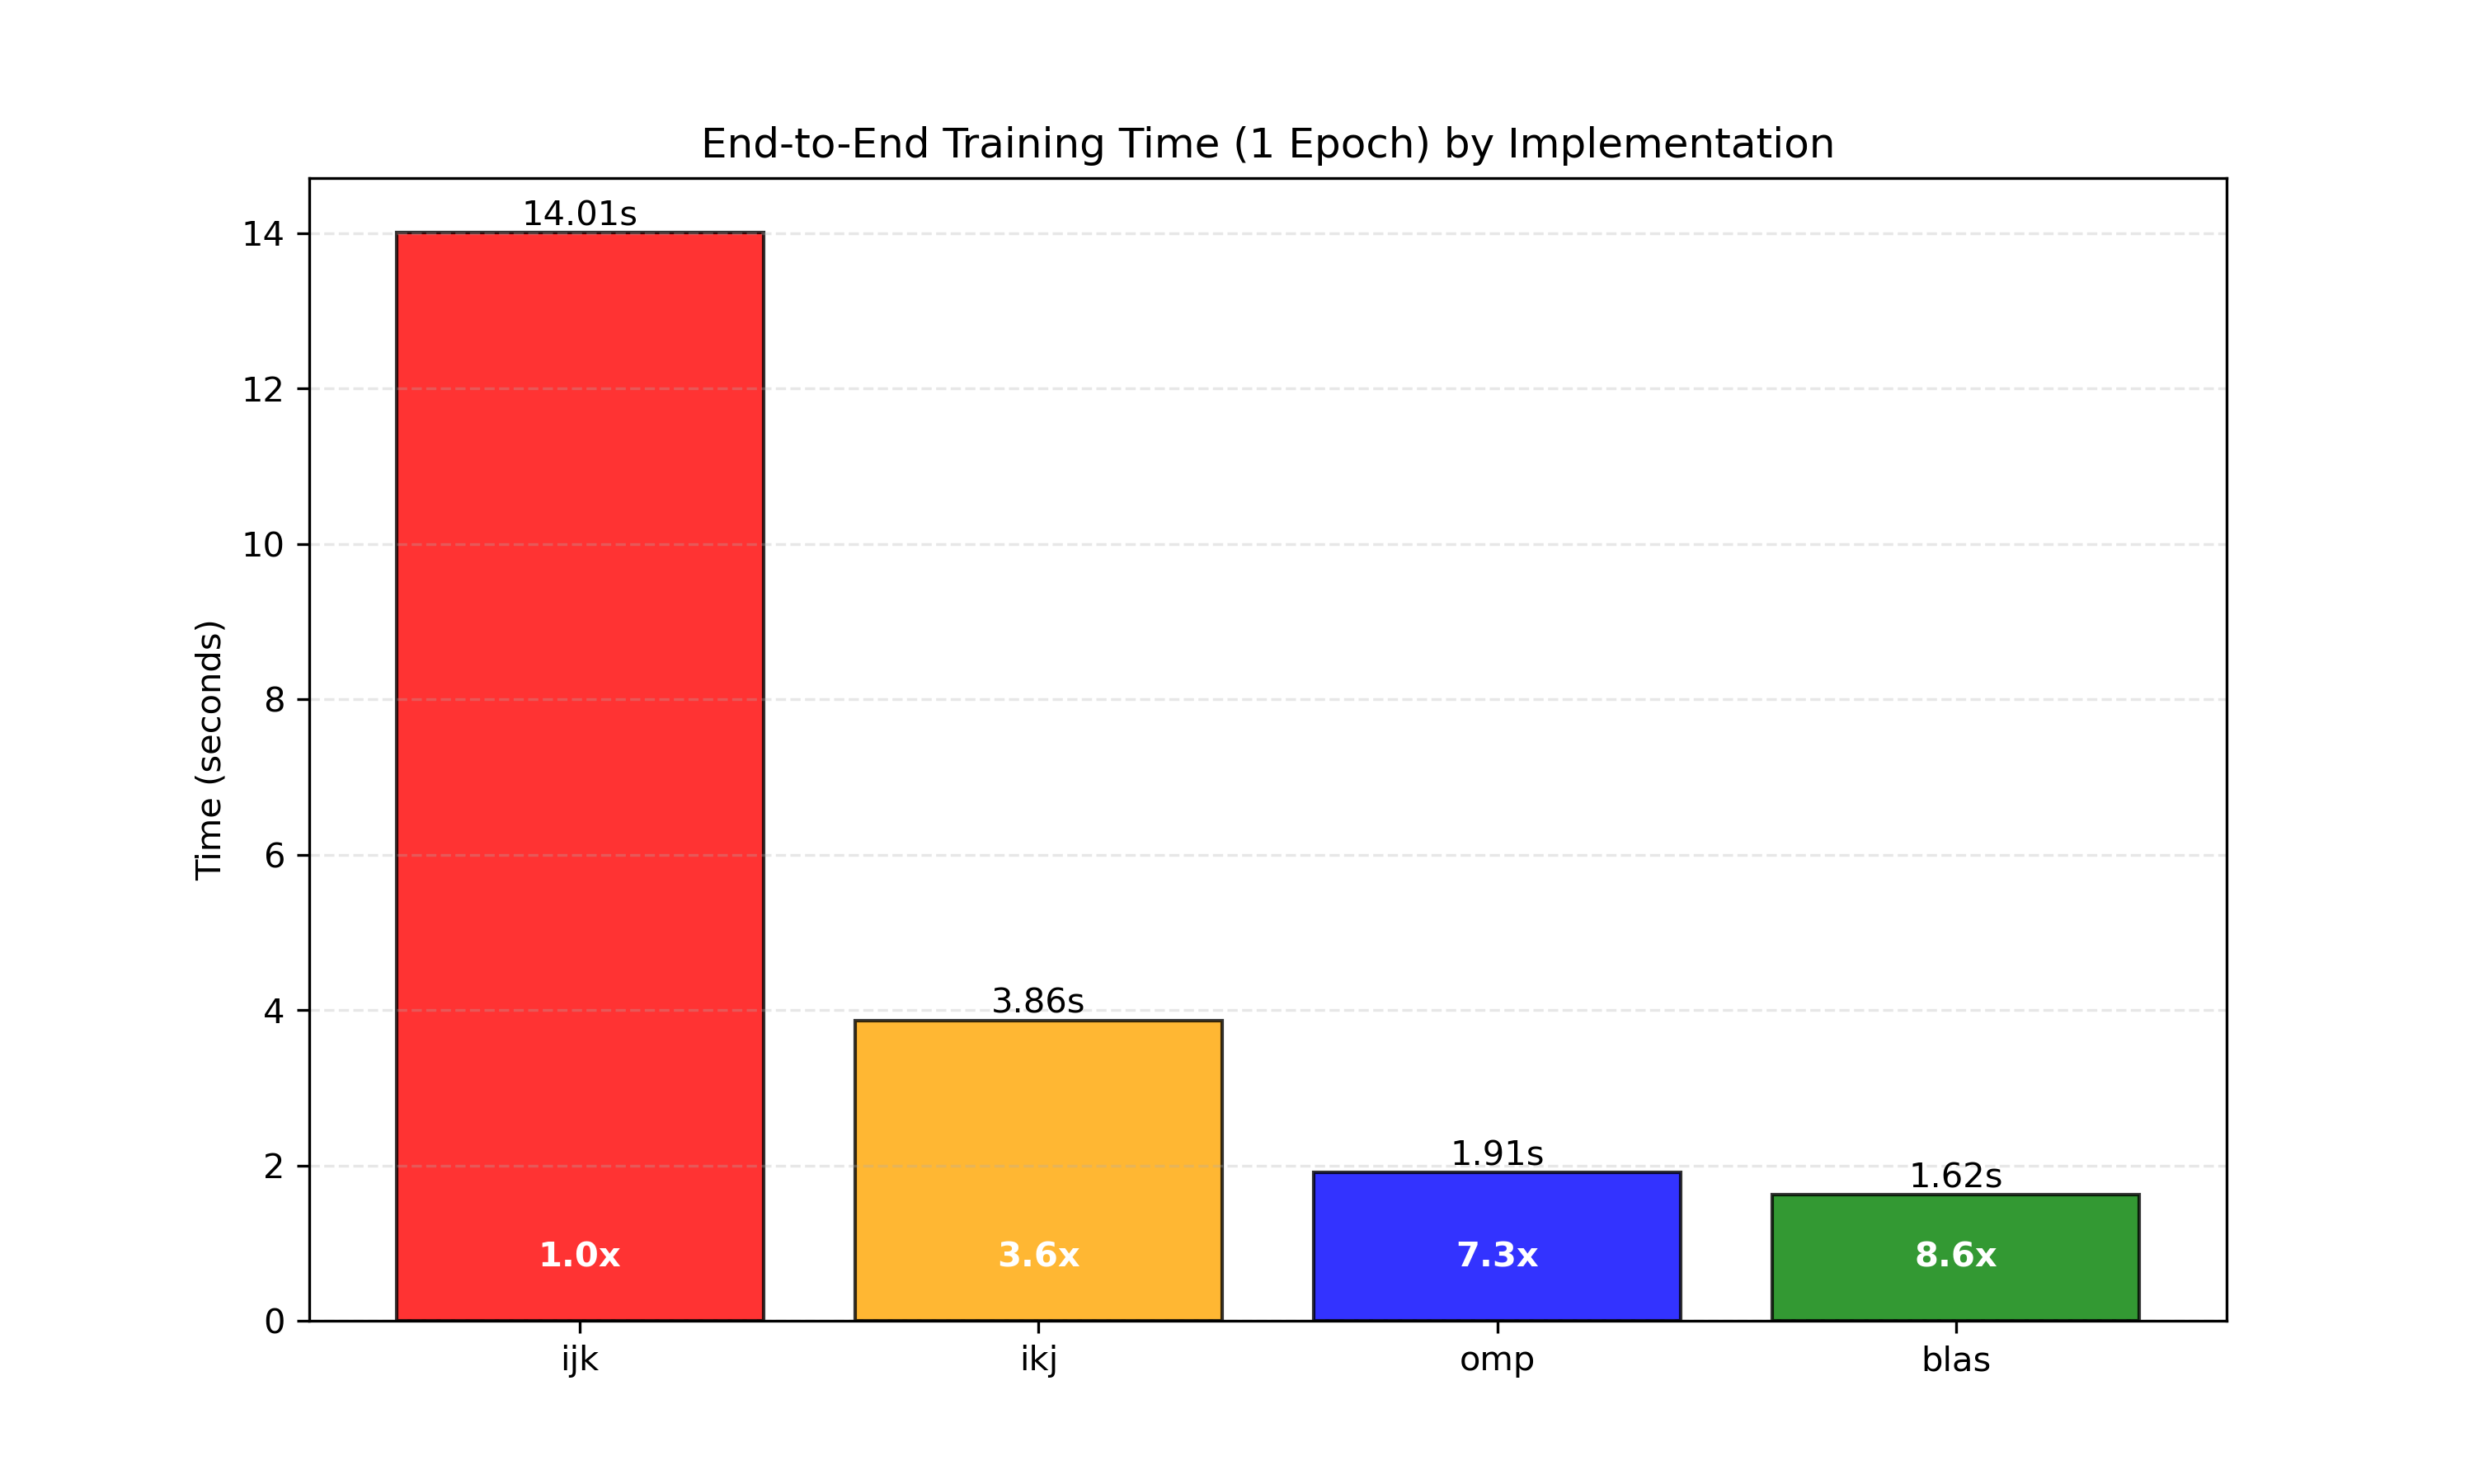
\includegraphics[width=\linewidth,height=0.42\textheight,keepaspectratio]{Images/e2e_benchmark_plot.png}
\vspace{-0.15cm}
{\scriptsize Répartition temps E2E}
\end{center}

\vspace{0.2cm}
\begin{alertblock}{\small Speedup Global}
\centering
\textbf{7.6×}\\
{\scriptsize Limité par I/O (Amdahl)}
\end{alertblock}
\end{columns}
\end{frame}

\begin{frame}{Convergence : premiers résultats}
\vspace{-0.2cm}
\begin{center}
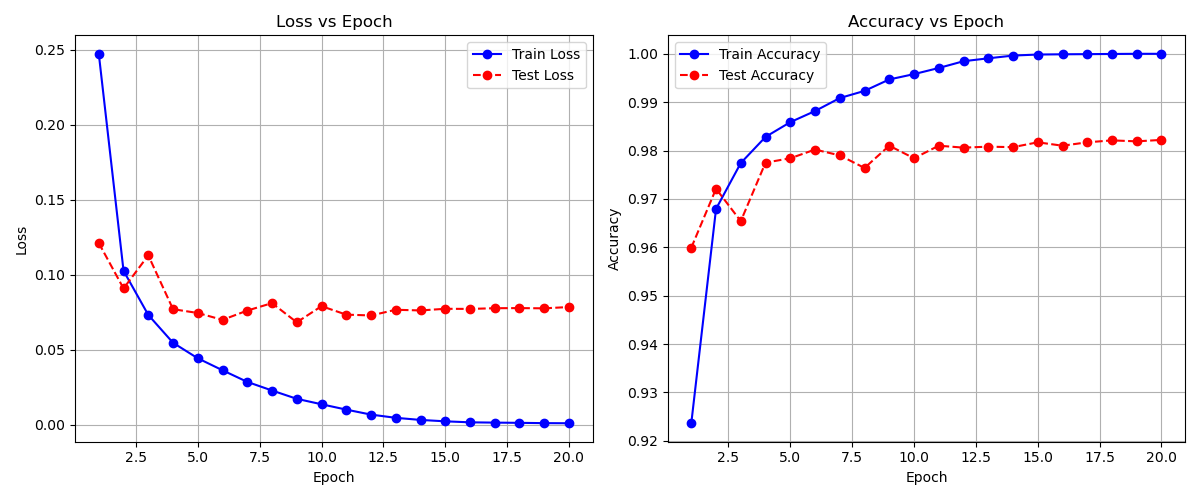
\includegraphics[width=0.8\textwidth,height=0.52\textheight,keepaspectratio]{Images/training_curve.png}
\vspace{-0.15cm}
{\scriptsize Loss et Accuracy (LR=0.01, Batch=64, Hidden=128, ReLU, 20 époques)}
\end{center}

\vspace{0.15cm}

{\small
\begin{columns}[c]
\column{0.33\textwidth}
\centering
\textbf{Précision finale}\\
\Large \textcolor{green}{$\sim$98.2\%}

\column{0.33\textwidth}
\centering
\textbf{Convergence}\\
Rapide et stable

\column{0.33\textwidth}
\centering
\textbf{Généralisation}\\
Écart train/val modéré
\end{columns}
}
\end{frame}

\begin{frame}{Impact du Learning Rate}
\begin{figure}
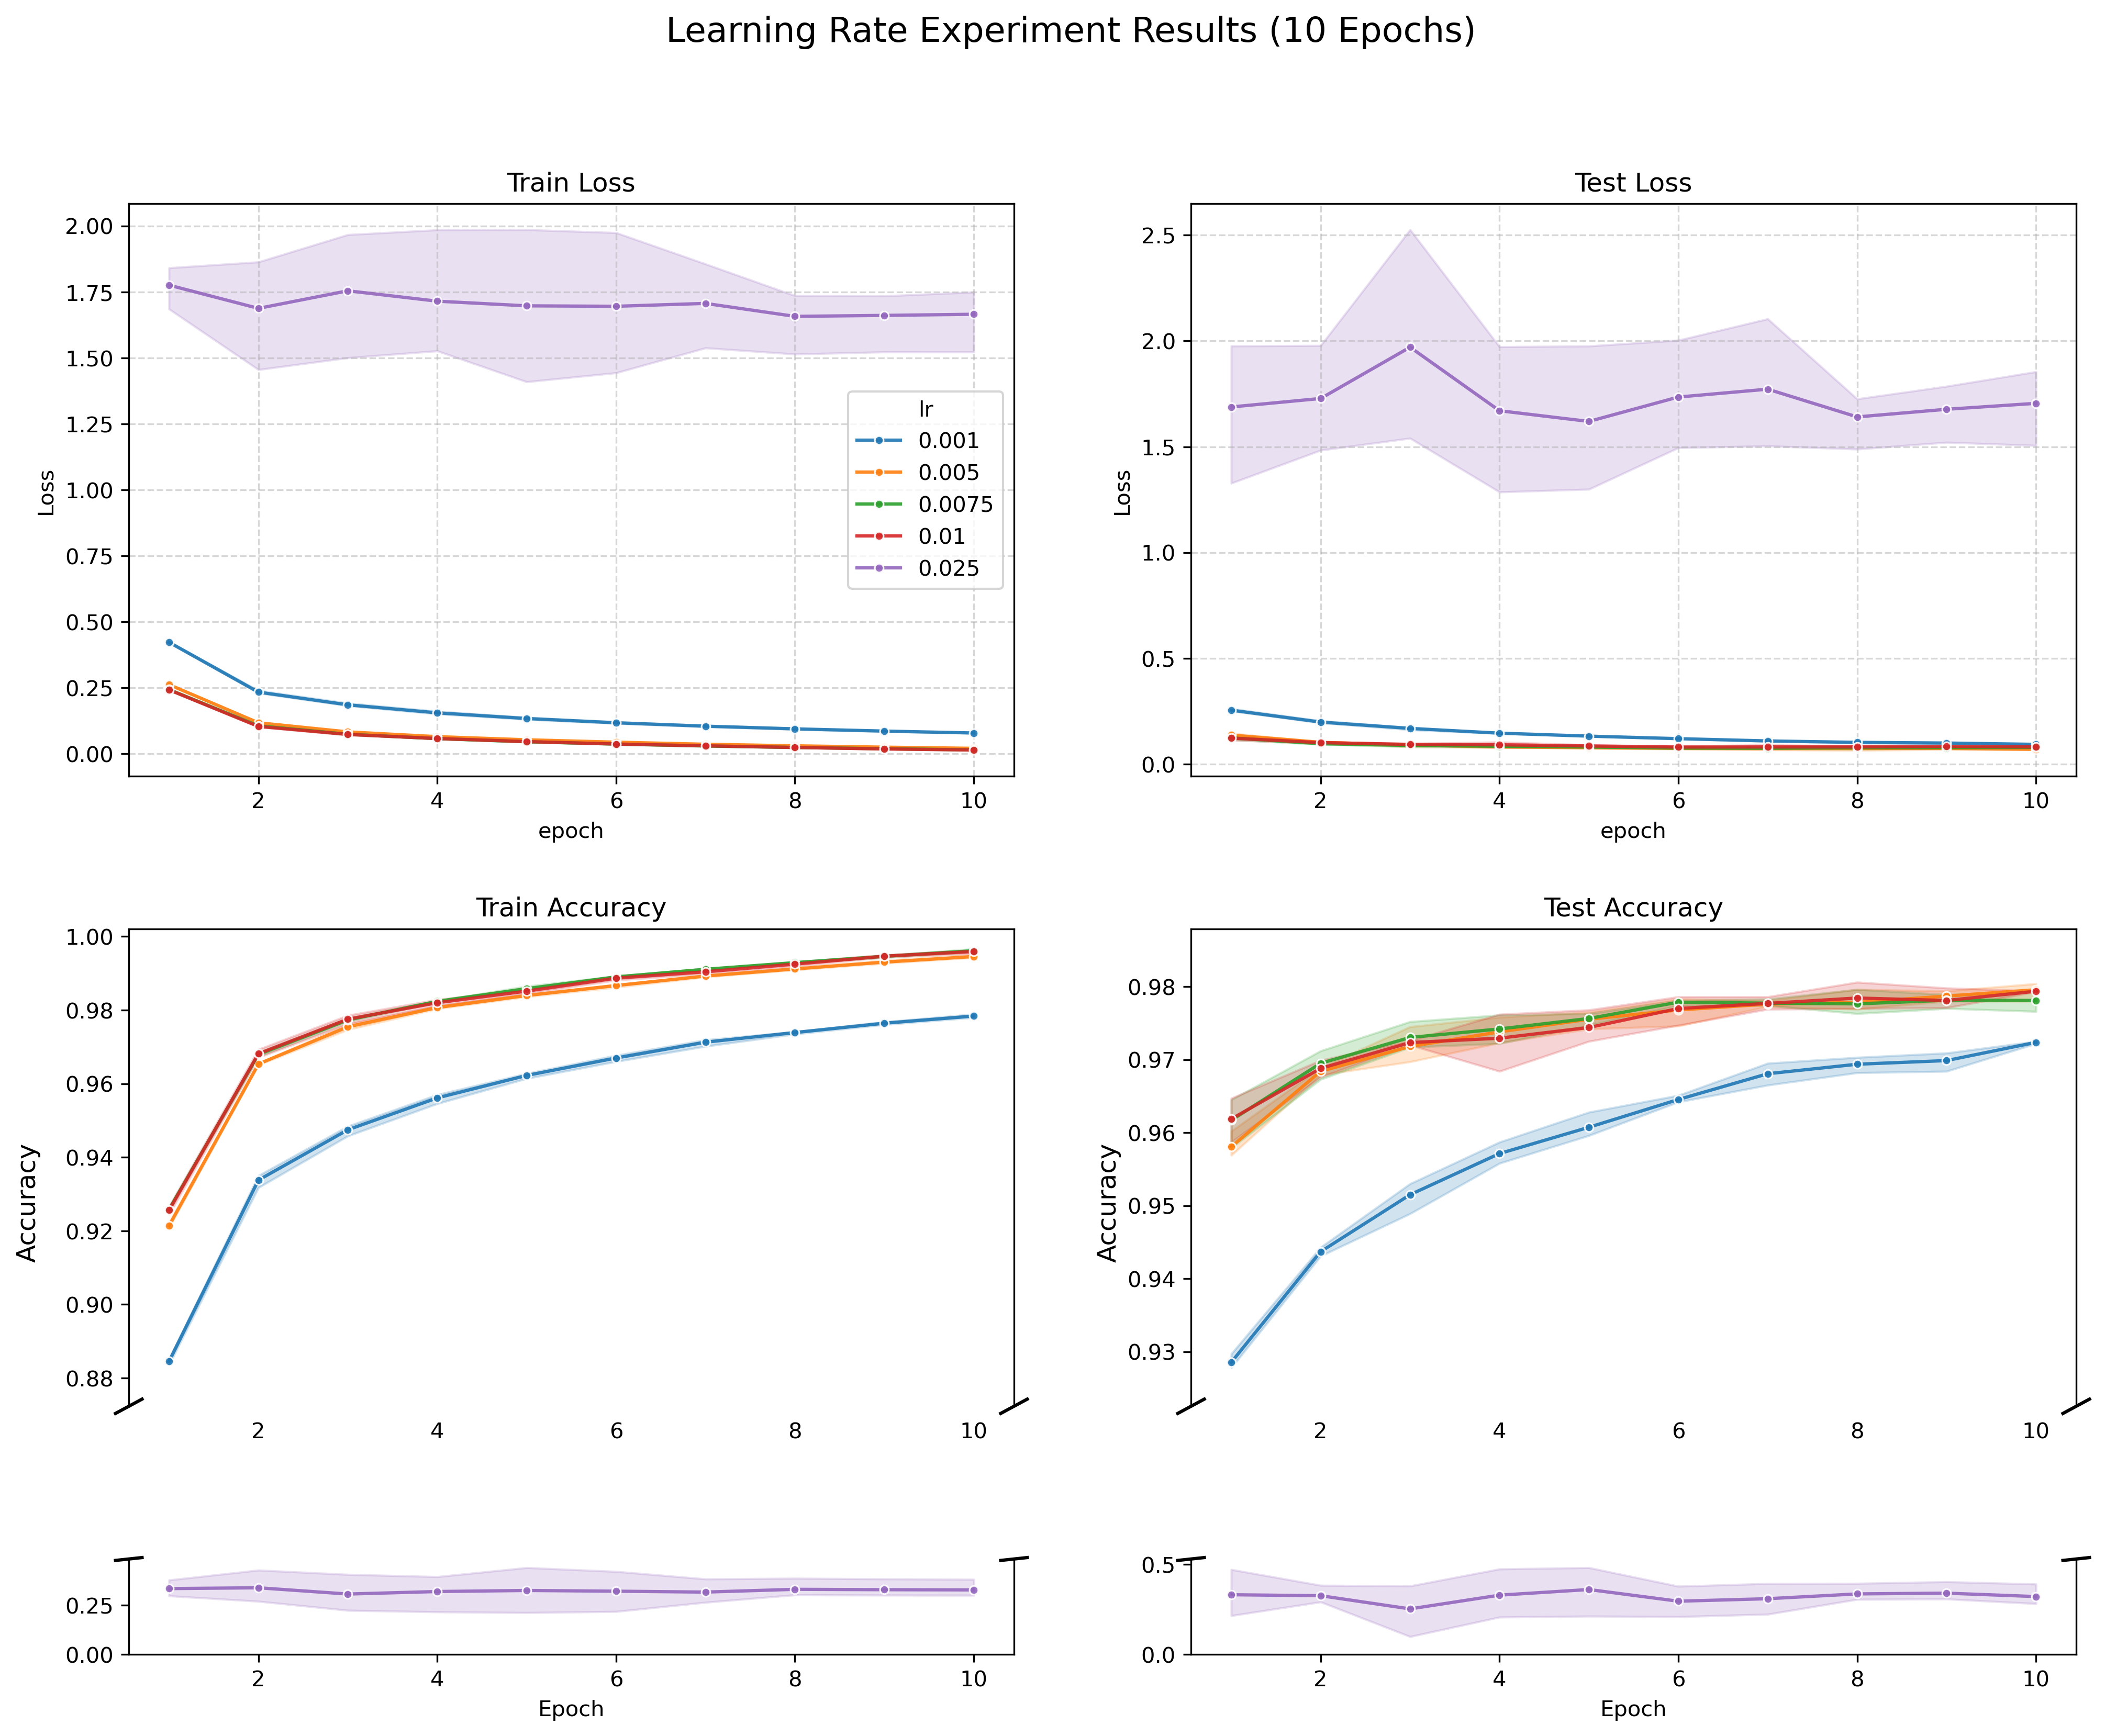
\includegraphics[width=0.85\textwidth,height=0.48\textheight,keepaspectratio]{Images/combined_lr_results.png}
\caption{Influence du taux d'apprentissage (10 époques, 3 graines)}
\end{figure}

\vspace{0.2cm}

\begin{itemize}
    \item \textbf{LR = 0.001} : Trop lent ($\sim$97.2\%)
    \item \textbf{LR $\in [0.005, 0.01]$} : \textcolor{green}{\textbf{Zone optimale}} ($\sim$98.0\%)
    \item \textbf{LR = 0.025} : \textcolor{red}{\textbf{Divergence}} ($\sim$32.1\%, variance élevée)
\end{itemize}
\end{frame}

\begin{frame}{Impact du Batch Size}
\begin{center}
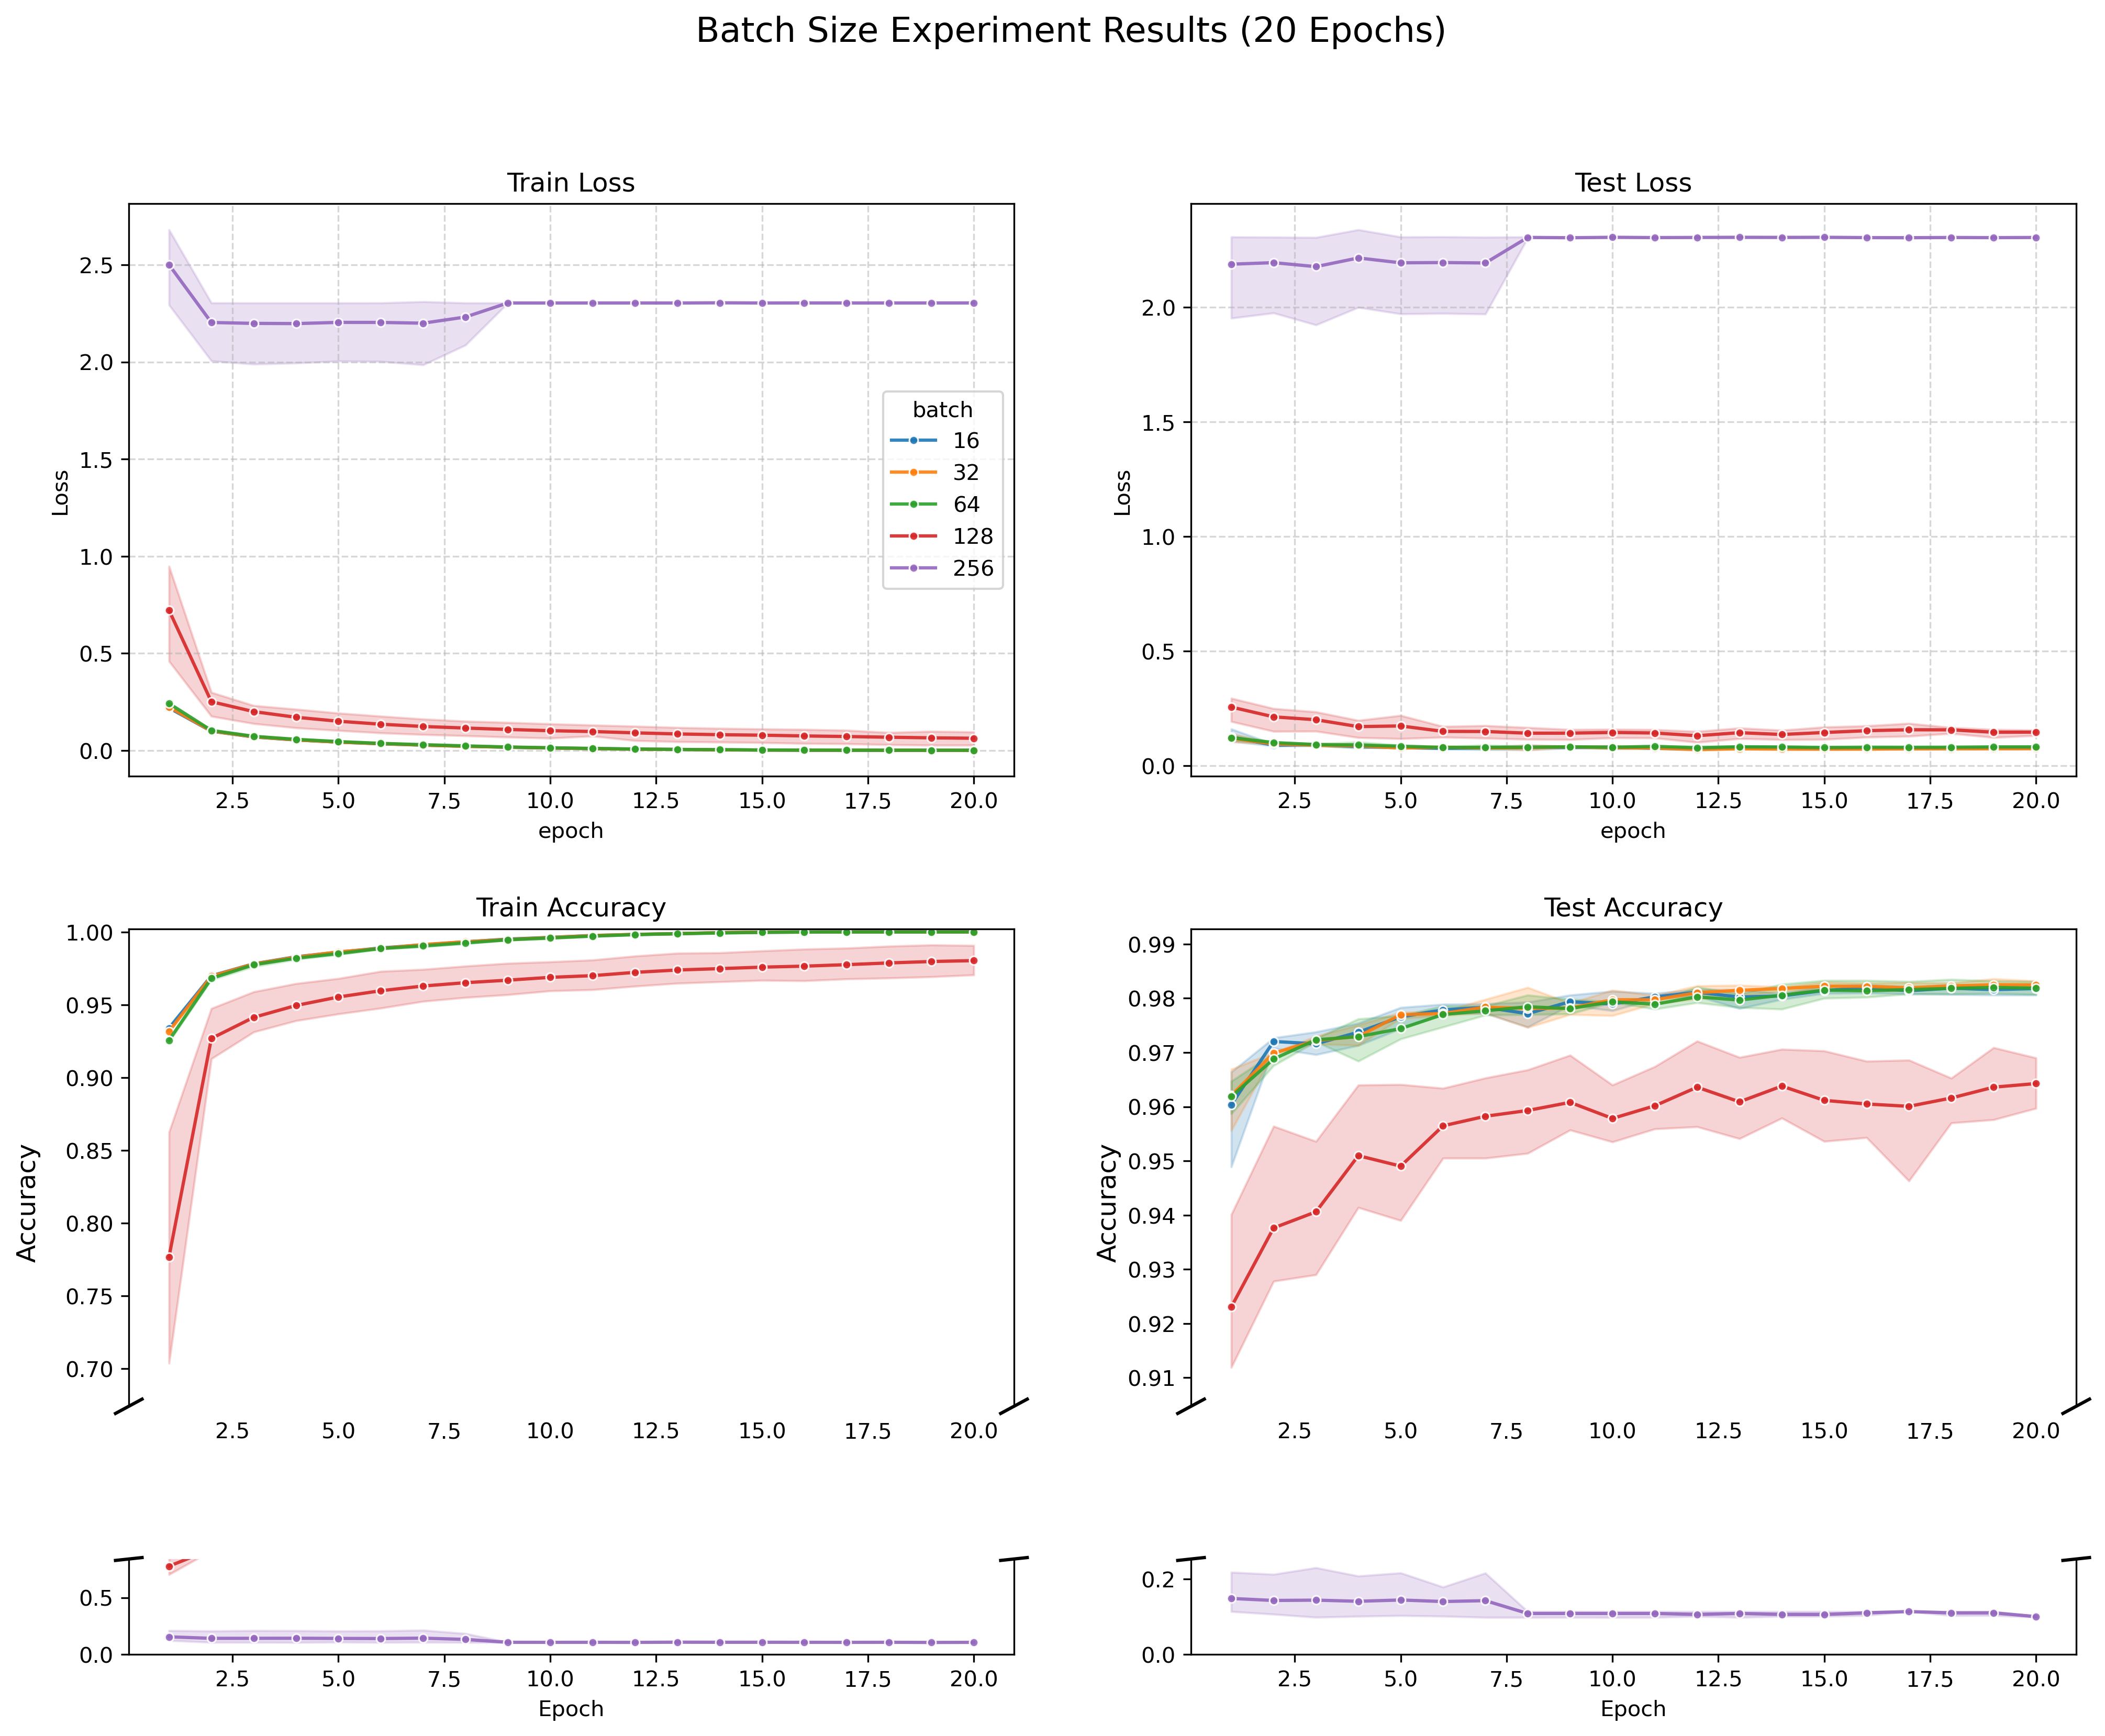
\includegraphics[width=0.88\textwidth,height=0.55\textheight,keepaspectratio]{Images/combined_batch_results.png}
\vspace{-0.2cm}
\small Influence de la taille de batch (20 époques, LR=0.01, 3 graines, Hidden=128)
\end{center}

\vspace{0.3cm}

\begin{columns}[T]
\column{0.33\textwidth}
\centering
\textbf{B $\in \{16, 32\}$}\\
Meilleur accuracy\\
Plus lent

\column{0.33\textwidth}
\centering
\textcolor{green}{\textbf{B = 64}}\\
\textcolor{green}{\textbf{Compromis optimal}}\\
\textcolor{green}{Précision + vitesse}

\column{0.33\textwidth}
\centering
\textcolor{red}{\textbf{B $\in \{128, 256\}$}}\\
\textcolor{red}{Dégradation}\\
\textcolor{red}{LR fixe inadapté}
\end{columns}
\end{frame}

\begin{frame}{Impact de la taille cachée et de l'activation}
\vspace{-0.2cm}
\begin{columns}[c]
\column{0.48\textwidth}
\begin{center}
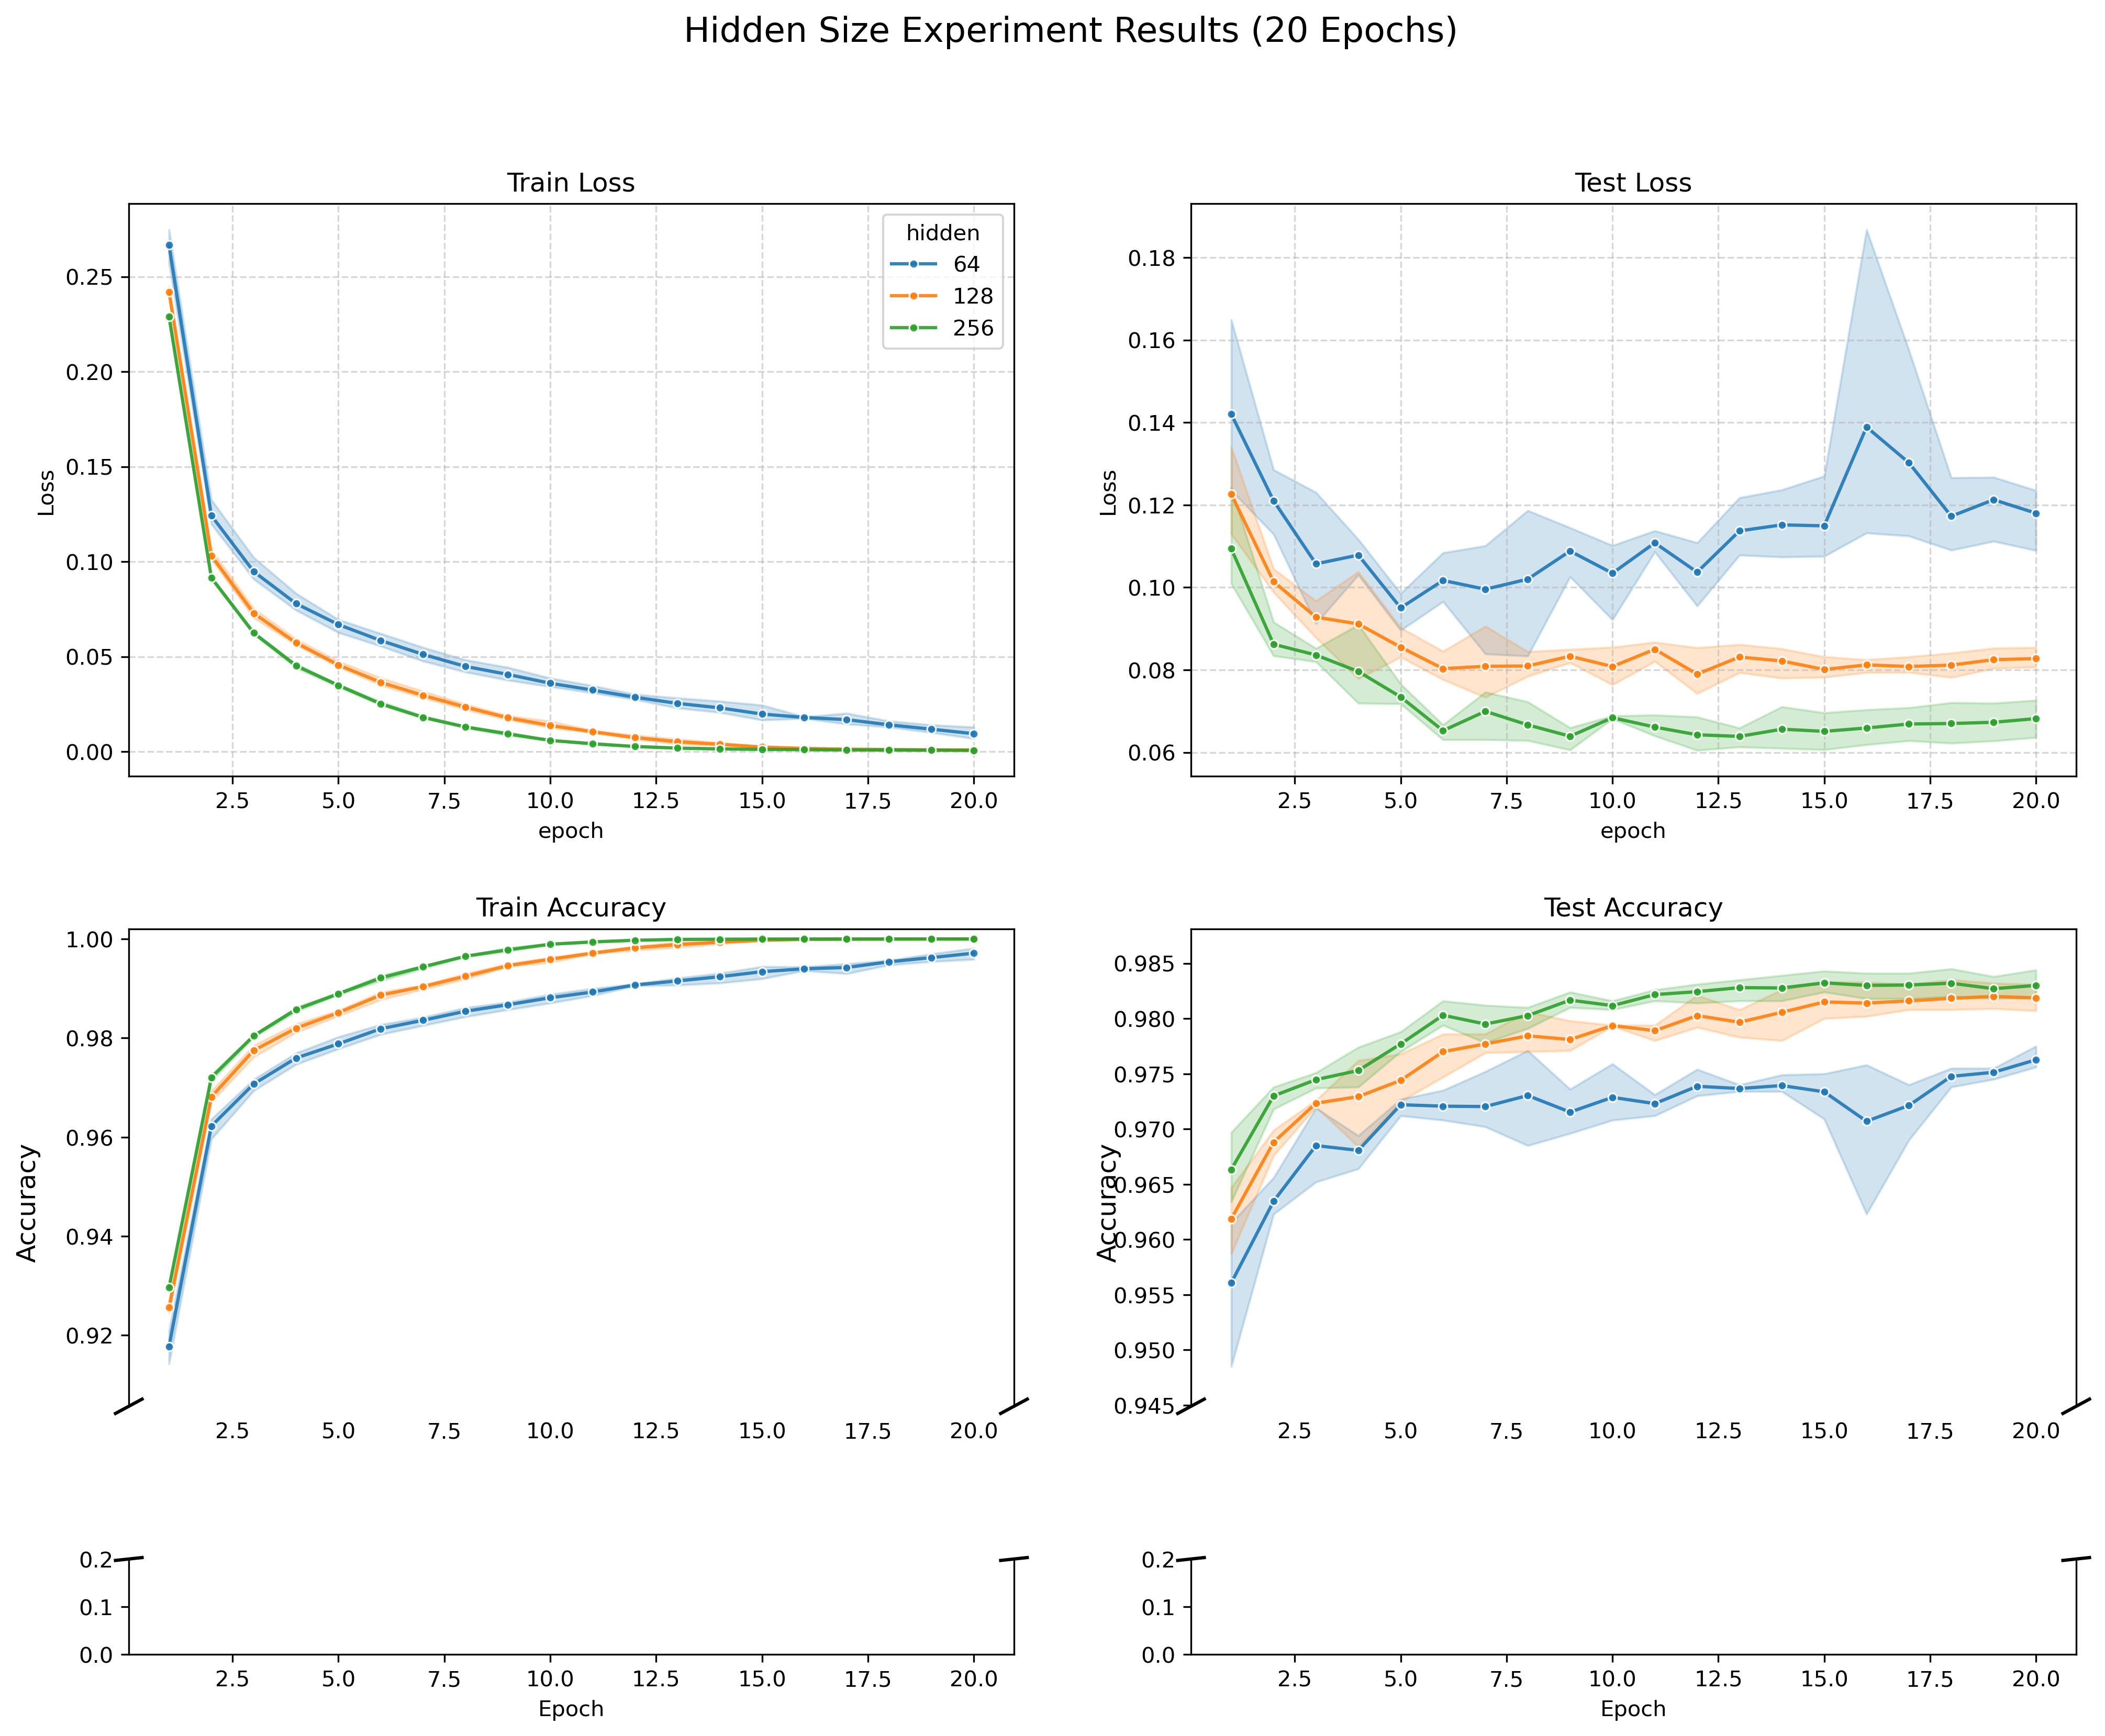
\includegraphics[width=\linewidth,height=0.42\textheight,keepaspectratio]{Images/combined_hidden_results.png}
\vspace{-0.15cm}
{\scriptsize Taille de couche cachée}
\end{center}

\vspace{0.15cm}
{\small
\textbf{Observations}
\begin{itemize}
    \item H=64 : Sous-apprentissage
    \item \textcolor{green}{\textbf{H=128 : Optimal}}
    \item H=256 : Gain marginal
\end{itemize}
}

\column{0.48\textwidth}
\begin{center}
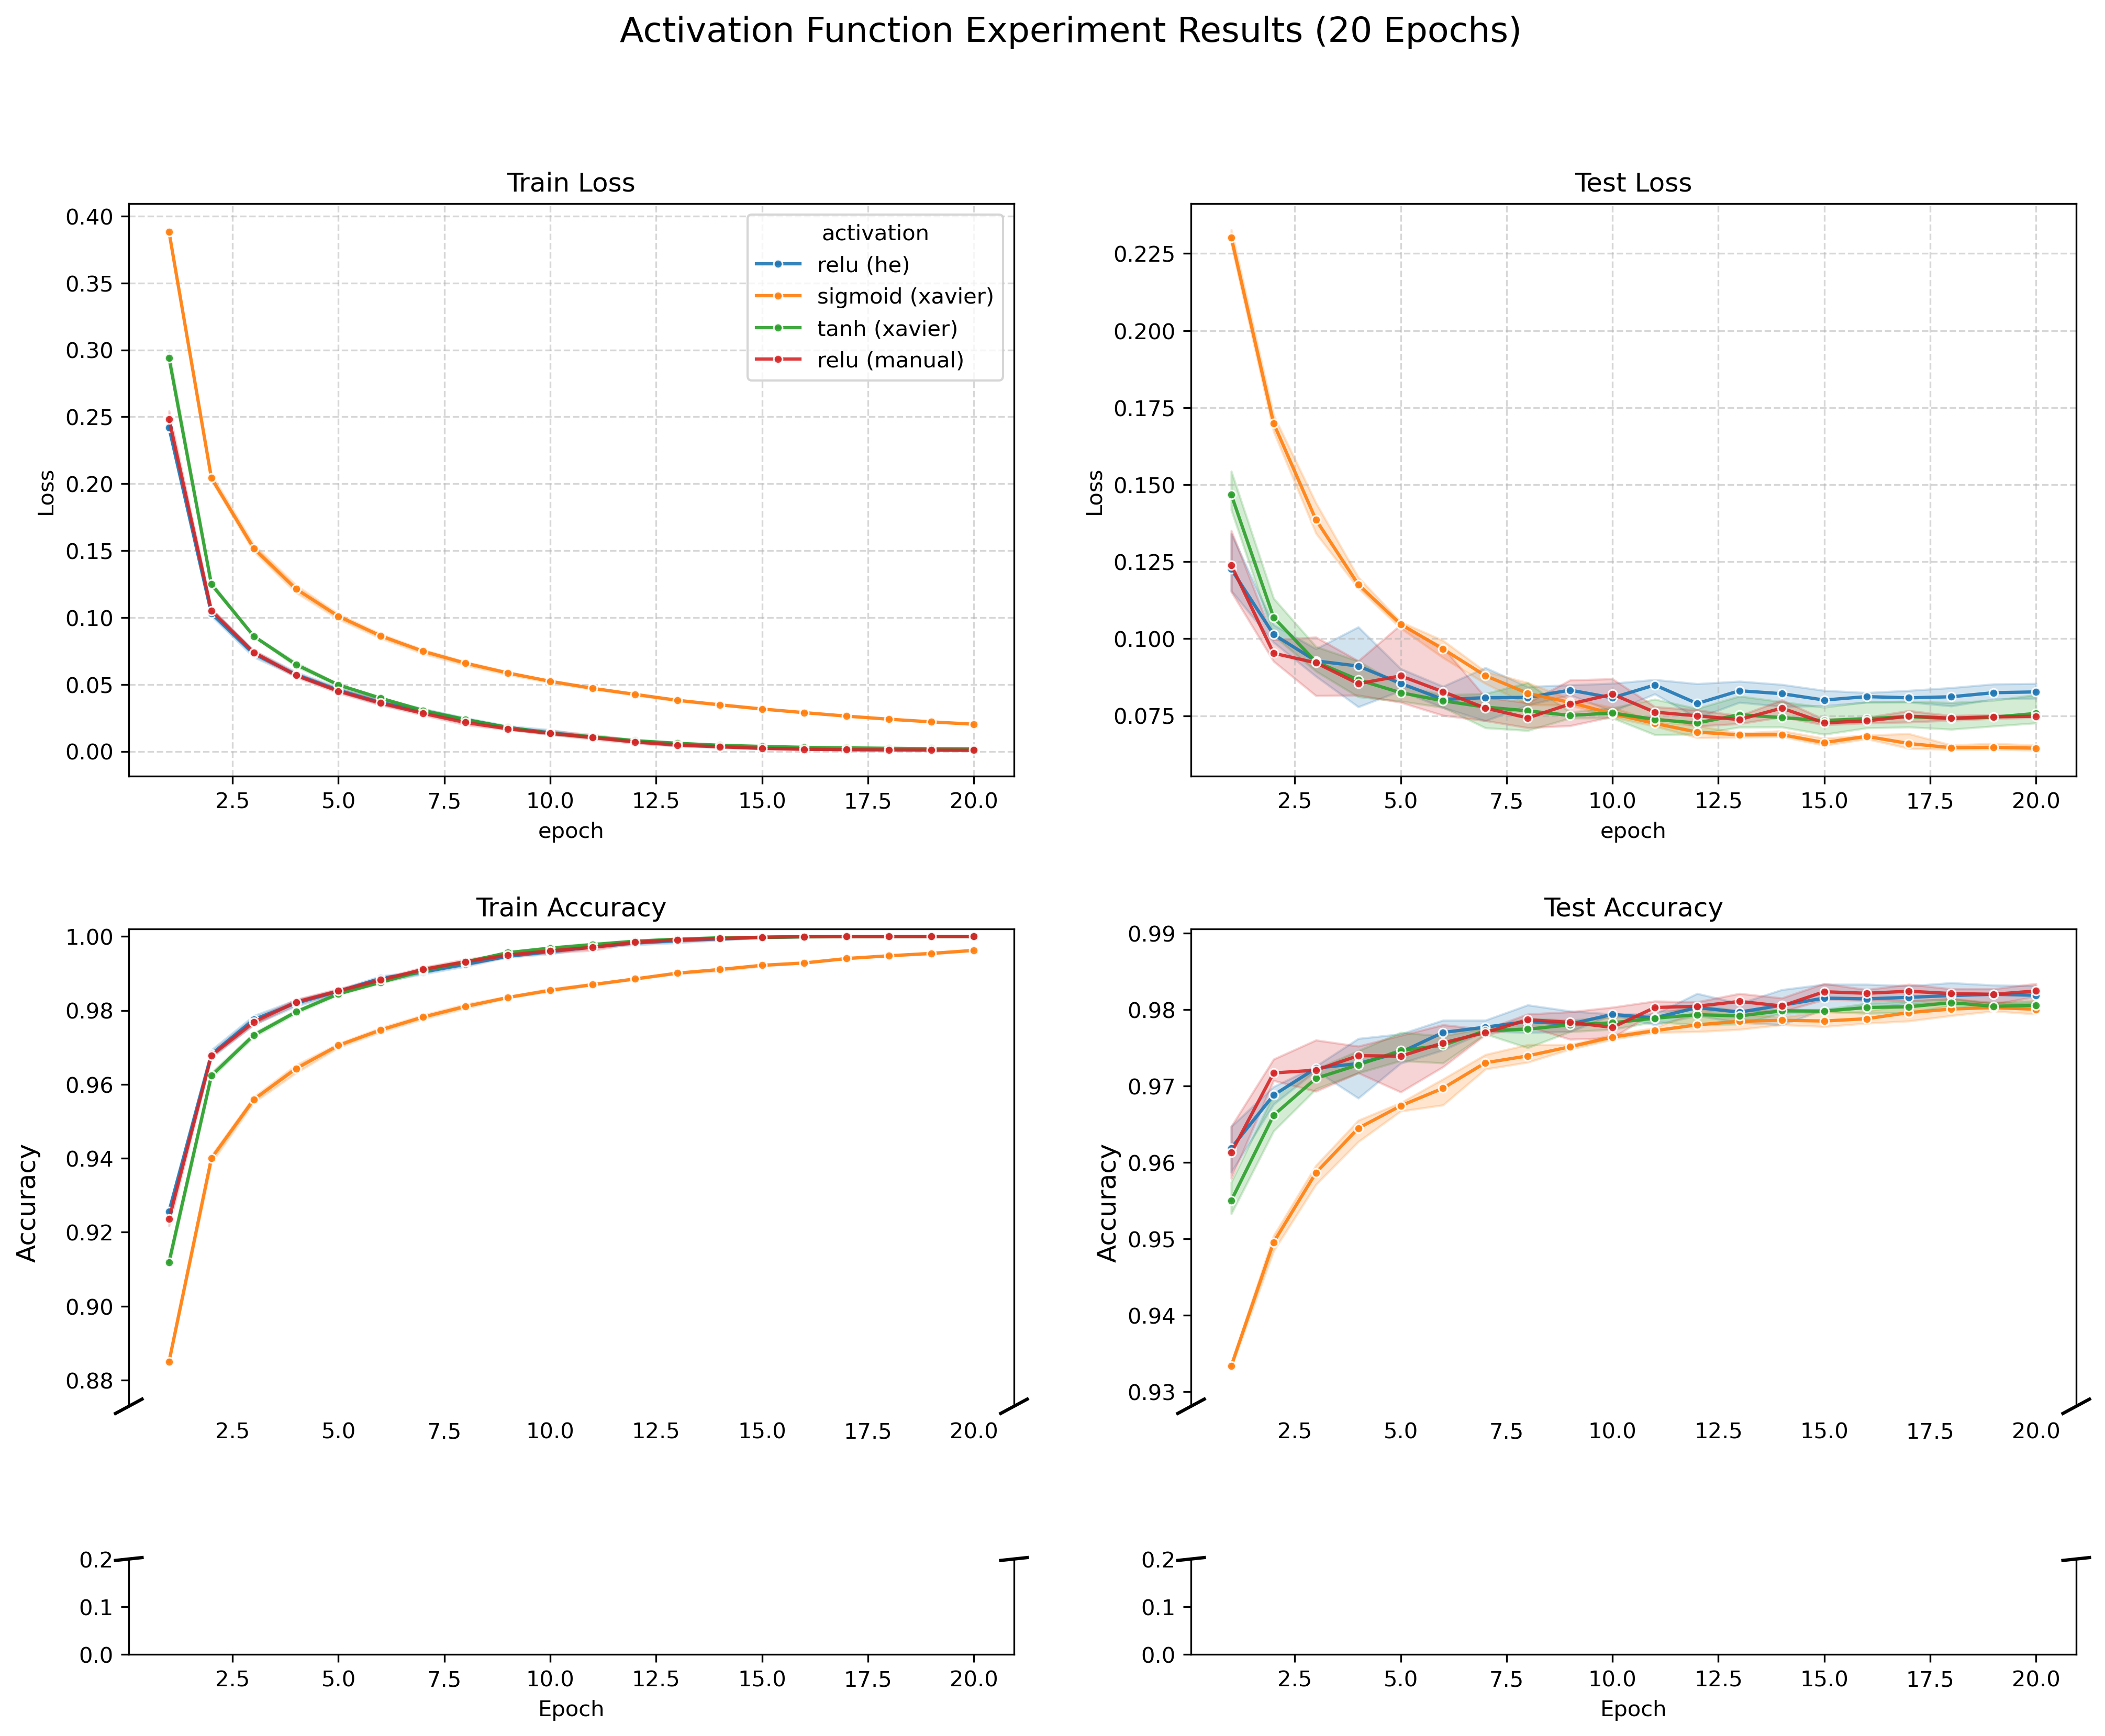
\includegraphics[width=\linewidth,height=0.42\textheight,keepaspectratio]{Images/combined_activation_results.png}
\vspace{-0.15cm}
{\scriptsize Fonctions d'activation}
\end{center}

\vspace{0.15cm}
{\small
\textbf{Résultats}
\begin{itemize}
    \item \textcolor{green}{\textbf{ReLU : Meilleur}}
    \item Tanh/Sigmoid : OK avec Xavier
\end{itemize}
}
\end{columns}
\end{frame}

\begin{frame}{Configuration optimale retenue}
\begin{center}
\begin{beamercolorbox}[rounded=true,shadow=true,wd=0.8\textwidth]{block body}
\Large
\vspace{0.3cm}
\textbf{Configuration finale}
\vspace{0.3cm}

\begin{tabular}{rl}
Learning Rate & : \textbf{0.01} \\
Batch Size & : \textbf{64} \\
Hidden Size & : \textbf{128} \\
Activation & : \textbf{ReLU} \\
Initialisation & : \textbf{He} \\
\end{tabular}

\vspace{0.3cm}
\textcolor{green}{\textbf{Précision validation : $\sim$98.2\%}}
\vspace{0.3cm}
\end{beamercolorbox}
\end{center}

\vspace{0.5cm}

\begin{itemize}
    \item Validation par Grid Search (3 graines par configuration)
    \item Équilibre entre performance et stabilité
    \item Temps d'entraînement raisonnable
\end{itemize}
\end{frame}

% ============================================================
\section{Organisation et Conclusion}
% ============================================================

\begin{frame}{Organisation du projet}
\begin{block}{Répartition des tâches}
\begin{itemize}
    \item \textbf{État de l'art} : Jianye, Hao, Xiang (collectif)
    \item \textbf{Conception} : Jianye (documentation, UML)
    \item \textbf{Prototype MLP} : Abdennour (tenseurs, couches, activations)
    \item \textbf{Moteur autodiff} : Hao + Xiang (graphe, opérations)
    \item \textbf{Intégration} : Jianye (pipeline complet, MNIST)
    \item \textbf{Entraînement} : Xiang (boucle), Jianye + Hao (optimizer, loss)
    \item \textbf{Optimisation HPC} : Jianye (profiling, benchmarks, Grid Search)
    \item \textbf{Rapport} : Collectif
\end{itemize}
\end{block}

\vspace{0.3cm}

\begin{alertblock}{Méthodologie}
Développement incrémental avec validation continue à chaque étape
\end{alertblock}
\end{frame}

\begin{frame}{Conclusion}
\begin{block}{Réalisations}
\begin{itemize}
    \item $\checkmark$ Implémentation complète \textbf{from scratch} en C++
    \item $\checkmark$ Moteur d'autodiff fonctionnel et élégant (DAG + lambdas)
    \item $\checkmark$ Validation ML : \textbf{$\sim$98.2\%} de précision sur MNIST
    \item $\checkmark$ Optimisation HPC : speedup \textbf{200×} sur le noyau de calcul
\end{itemize}
\end{block}

\vspace{0.3cm}

\begin{alertblock}{Enseignements clés}
\begin{itemize}
    \item \textbf{Dual challenge} : algorithmique (convergence) + computationnel (performance)
    \item \textbf{Loi d'Amdahl} : après optimisation du calcul, les I/O deviennent le goulot
    \item \textbf{Importance du protocole} : mesures reproductibles essentielles
\end{itemize}
\end{alertblock}
\end{frame}

\begin{frame}{Perspectives}
\begin{columns}[T]
\column{0.5\textwidth}
\textbf{Extensions ML}
\begin{itemize}
    \item Optimiseurs avancés (Momentum, Adam)
    \item Régularisation (L2, Dropout)
    \item Architectures CNN
    \item Datasets plus complexes
\end{itemize}

\vspace{0.3cm}
\textbf{Optimisations HPC}
\begin{itemize}
    \item Support GPU (CUDA)
    \item Vectorisation explicite (AVX-512)
    \item Memory pool / arenas
\end{itemize}

\column{0.5\textwidth}
\textbf{Parallélisme à l'échelle}
\begin{itemize}
    \item Data parallelism (MPI)
    \item Model parallelism
    \item Pipeline de données optimisé
\end{itemize}

\vspace{0.3cm}
\textbf{Reproductibilité}
\begin{itemize}
    \item Framework de benchmarking
    \item CI/CD pour validation
    \item Documentation utilisateur
\end{itemize}
\end{columns}

\vspace{0.5cm}
\begin{center}
\textbf{Projet complet disponible sur} \texttt{[lien GitHub]}
\end{center}
\end{frame}

\begin{frame}[plain]
\Huge Merci de votre attention !

\vspace{1cm}
\Large Questions ?
\end{frame}

% Slides de backup
\appendix

\begin{frame}[allowframebreaks,fragile]{Détails techniques : Matrix operations}
\textbf{Implémentation du produit matriciel}

\begin{lstlisting}[language=C++]
// Version naive (ijk) - mauvaise localite cache
for (int i = 0; i < m; ++i)
    for (int j = 0; j < p; ++j)
        for (int k = 0; k < n; ++k)
            C(i,j) += A(i,k) * B(k,j);

// Version reordonnee (ikj) - meilleure localite
for (int i = 0; i < m; ++i)
    for (int k = 0; k < n; ++k)
        for (int j = 0; j < p; ++j)
            C(i,j) += A(i,k) * B(k,j);

// Version OpenMP
#pragma omp parallel for
for (int i = 0; i < m; ++i)
    for (int k = 0; k < n; ++k)
        for (int j = 0; j < p; ++j)
            C(i,j) += A(i,k) * B(k,j);
\end{lstlisting}
\end{frame}

\begin{frame}{Détails techniques : Backward pass}
\textbf{Exemple de calcul de gradient (LinearLayer)}

\begin{align*}
\text{Forward:} \quad & Y = XW + b \\
\text{Backward:} \quad & \frac{\partial L}{\partial X} = \frac{\partial L}{\partial Y} \cdot W^T \\
& \frac{\partial L}{\partial W} = X^T \cdot \frac{\partial L}{\partial Y} \\
& \frac{\partial L}{\partial b} = \sum \frac{\partial L}{\partial Y}
\end{align*}

\vspace{0.5cm}

\textbf{Implémentation}
\begin{itemize}
    \item Stockage de $X$ pendant le forward
    \item Calcul des trois gradients lors du backward
    \item Accumulation dans les nœuds parents
\end{itemize}
\end{frame}

\end{document}
